\documentclass[conference]{IEEEtran}

\usepackage[spanish]{babel}
\usepackage[utf8]{inputenc}
\usepackage{cite}
\usepackage{amsmath, amsthm,amssymb,amsfonts}
\usepackage{algorithmic}
\usepackage{graphicx}
\usepackage{textcomp}
\usepackage{xcolor}
\def\BibTeX{{\rm B\kern-.05em{\sc i\kern-.025em b}\kern-.08em
    T\kern-.1667em\lower.7ex\hbox{E}\kern-.125emX}}

% Definición del entorno 'definition'
\newtheorem{definition}{Definición}

\begin{document}
\title{Trajectory Tracking in Autonomous Drone Racing Using Model Predictive Control
	% {\footnotesize \textsuperscript{*}Note: Sub-titles are not captured in Xplore and
	% should not be used}
	% \thanks{Identify applicable funding agency here. If none, delete this.}
}

\author{
	\IEEEauthorblockN{José Alejandro León Sánchez}
	\IEEEauthorblockA{\textit{Posgrado de Ingeniería} \\
		\textit{UNAM}\\
		CDMX, Mexico}
	\and
	\IEEEauthorblockN{Alejandro Gutiérrez-Gil}
	\IEEEauthorblockA{\textit{INAOEP} \\
		\textit{CONAHCYT}\\
		Puebla, Mexico}
}

\maketitle

\begin{abstract}
    En esta ponencia se presentan los avances en el uso de Model Predictive Control (MPC) para el seguimiento de trayectorias en drones autónomos. A través de un modelado preciso y técnicas de optimización, se demuestra la capacidad de MPC para predecir y ajustar dinámicamente las acciones de control en aplicaciones de alta velocidad, como las carreras autónomas de drones. También se introduce un controlador neuronal basado en redes profundas, capaz de generalizar trayectorias complejas mediante el aprendizaje de controladores clásicos.
\end{abstract}

\begin{IEEEkeywords}
    Control predictivo, drones autónomos, seguimiento de trayectorias, redes neuronales, optimización en tiempo real.
\end{IEEEkeywords}

\subsection*{Introducción}

El Model Predictive Control (MPC) es un enfoque avanzado de control óptimo basado en modelos, ampliamente utilizado en aplicaciones donde la precisión y la adaptabilidad son fundamentales. Este método se distingue por su capacidad de prever la evolución futura del sistema, recalcular dinámicamente las acciones de control en tiempo real y operar en sistemas con baja latencia. Durante la ponencia, el Dr. Alejandro Gutiérrez-Giles destacó las ventajas clave de MPC, como su capacidad para abordar restricciones físicas y operativas del sistema. Matemáticamente, el MPC minimiza una función de costo definida en un horizonte de predicción finito, sujeta a las ecuaciones dinámicas del sistema y a restricciones de estado y entrada.

\begin{figure}[h]
    \centering
    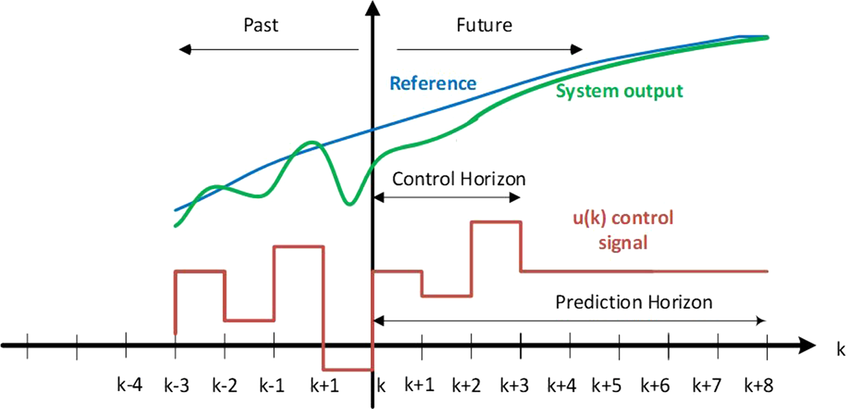
\includegraphics[width=0.5\textwidth]{predictionHorizon.png}
    \caption{Representación del horizonte de predicción en MPC.}
\end{figure}

\subsection*{Modelado del Cuadrotor}

El cuadrotor se modela utilizando un enfoque basado en coordenadas generalizadas y dinámica newtoniana. Las coordenadas $\zeta = [x, y, z]^T$ representan la posición del cuadrotor en el espacio tridimensional, mientras que $\eta = [\phi, \theta, \psi]^T$ describe las orientaciones en términos de ángulos de roll, pitch y yaw. Estas variables, combinadas en $q = [\zeta, \eta]^T$, permiten describir completamente el estado del sistema.

Las velocidades lineales en el marco del cuerpo, $V_B = [v_{x,B}, v_{y,B}, v_{z,B}]^T$, y las velocidades angulares, $v = [p, q, r]^T$, también se incorporan en el modelo. La matriz de rotación $R_B$ se utiliza para transformar entre los marcos de referencia inercial y del cuerpo, mientras que el tensor de inercia $I$ caracteriza la resistencia rotacional del cuadrotor.

\subsection*{Arquitectura Cerrada de Control}

En algunos cuadrotores comerciales, el control directo de los rotores no es posible. En su lugar, se emplea un controlador de vuelo que recibe como entradas la aceleración (throttle) y los ángulos de roll, pitch y yaw. Este controlador también compensa la gravedad y utiliza mediciones de velocidades lineales y angulares para garantizar una operación estable. El diseño del MPC presentado por el Dr. Gutiérrez-Giles utiliza una función de costo cuadrática que penaliza tanto las desviaciones del estado deseado como el uso excesivo de las entradas de control. Las restricciones del modelo se formulan en tiempo discreto para garantizar una implementación eficiente.

\subsection*{Planificación de Trayectorias}

La planificación de trayectorias es un componente clave para el éxito en escenarios de competencia como las carreras autónomas de drones. En este caso, el Dr. Gutiérrez-Giles presentó un enfoque basado en polinomios interpoladores de tercer orden para generar trayectorias suaves entre puntos clave, como las ubicaciones de las puertas de paso. Este método garantiza la continuidad en las posiciones y velocidades, y optimiza el tiempo mediante parametrización por longitud de arco. Para calcular la longitud de arco y resolver la parametrización temporal, se utilizaron métodos numéricos, lo que permite obtener trayectorias optimizadas en tiempo real.

El horizonte de predicción utilizado en las simulaciones fue de 50 pasos, con un intervalo de muestreo $T_s$ de 20 ms, mientras que el horizonte de control se estableció en 10 pasos. Además, se empleó un filtro de Kalman para estimar las velocidades a partir de mediciones ruidosas.

\subsection*{Controlador Neuronal End-to-End}

El enfoque del controlador neuronal presentado como extensión del MPC, denominado \textit{DeepPilot}, utiliza una red neuronal entrenada con 5885 imágenes mosaico generadas a partir de cámaras a bordo del cuadrotor. Este controlador fue diseñado para incorporar la temporalidad y fue capaz de aprender las reglas del control clásico mientras generalizaba a trayectorias más complejas. Las simulaciones demostraron su eficacia en escenarios donde el MPC tradicional podría ser limitado por los modelos dinámicos.

\subsection*{Conclusiones}

El trabajo presentado demuestra la efectividad del MPC en el seguimiento de trayectorias en tiempo mínimo y su integración con arquitecturas cerradas de control para cuadrotores. Además, el controlador neuronal mostró ser una herramienta poderosa para generalizar el comportamiento del cuadrotor a trayectorias no vistas previamente. Las líneas de investigación futuras incluyen mejorar el desempeño del controlador neuronal, realizar validaciones experimentales y explorar el uso exclusivo de sensores y procesamiento a bordo.

\end{document}